\subsection{Relationen}
Eine \emph{Relation} von \(A\) nach \(B\) ist ein Tripel
\[
R=(G,A,B)
\]
wobei \(A\) die Quellmenge, \(B\) die Zielmenge und \(G\subseteq A\times B\) der \emph{Graph} von \(R\) ist. Ist \(A=B\), so heisst \(R\) \emph{homogen} auf \(A\).

\subsubsection{Notation}
Sei \(R=(G,A,B)\) eine Relation von \(A\) nach \(B\).
\begin{itemize}
  \item Ist \(G\) der Graph von \(R\), so schreibt man \(G_R\)
  \item Ist \((x,y)\in G\), dann schreibt man \(xRy\) (\(x\) steht in Relation zu \(y\) bezüglich \(R\)).
  \item Sind \(A\) und \(B\) Teilmengen von \(\mathbb{R}\), so kann man \(R\) auch als Menge von Punkten in der Ebene darstellen: \(\{(x,y)\mid xRy\}\).\\
    % 1. x^2 = y^2
    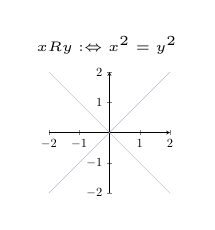
\begin{tikzpicture}[scale=.45]
      \begin{axis}[axis lines=middle, xmin=-2, xmax=2, ymin=-2, ymax=2, width=5cm, height=5cm]
        \addplot[domain=-3:3, samples=100, blue!30] {x};
        \addplot[domain=-3:3, samples=100, blue!30] {-x};
      \end{axis}
      \node[anchor=south] at (current bounding box.north) {\tiny{$xRy: \Leftrightarrow x^2 = y^2$}};
    \end{tikzpicture}
    % 2. x^2 + y^2 = 1
    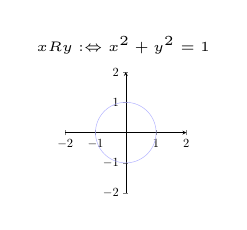
\begin{tikzpicture}[scale=.45]
      \begin{axis}[axis lines=middle, xmin=-2, xmax=2, ymin=-2, ymax=2, width=5cm, height=5cm]
        \addplot[domain=0:360, samples=200, blue!30] ({cos(x)}, {sin(x)});
      \end{axis}
      \node[anchor=south] at (current bounding box.north) {\tiny{$xRy: \Leftrightarrow x^2 + y^2 = 1$}};
    \end{tikzpicture}
  \item Als gerichteter Graph: Elemente von \(A\) und \(B\) als Knoten; für jedes \((x,y)\in G\) ein Pfeil \(x\to y\).\\
    \begin{tikzpicture}[main/.style = {draw, circle}] 
      \node[main] (1) {$1$}; 
      \node[main] (2) [right=0.5cm of 1] {$2$}; 
      \node[main] (3) [below=0.5cm of 1] {$3$}; 
      \node[main] (4) [right=0.5cm of 3] {$4$};
      \draw[->] (1) to (2);
      \draw[->] (1) to (3);
      \draw[->] (1) to (4);
      \draw[->] (2) to (4);
      \draw[->] (1) to [out=90,in=140,looseness=4] (1);
      \draw[->] (2) to [out=90,in=140,looseness=4] (2);
      \draw[->] (3) to [out=180,in=230,looseness=4] (3);
      \draw[->] (4) to [out=180,in=230,looseness=4] (4);
      \node[anchor=south] at (current bounding box.north) {\tiny{$xRy: \Leftrightarrow x \text{ teilt } y$}};
    \end{tikzpicture}
    \begin{tikzpicture}[main/.style = {draw, circle}] 
      \node[main] (1) {$1$}; 
      \node[main] (2) [right=0.5cm of 1] {$2$}; 
      \node[main] (3) [below=0.5cm of 1] {$3$}; 
      \node[main] (4) [right=0.5cm of 3] {$4$};
      \draw[<->] (1) to (3);
      \draw[<->] (2) to (4);
      \draw[->] (1) to [out=90,in=140,looseness=4] (1);
      \draw[->] (2) to [out=90,in=140,looseness=4] (2);
      \draw[->] (3) to [out=180,in=230,looseness=4] (3);
      \draw[->] (4) to [out=180,in=230,looseness=4] (4);
      \node[anchor=south] at (current bounding box.north) {\tiny{$xRy: \Leftrightarrow x+y \text{ ist gerade}$}};
    \end{tikzpicture} 
\end{itemize}

\subsubsection{Domäne}
Die Domäne und das Bild einer Relation geben an, welche Elemente der Quell- bzw. Zielmenge tatsächlich in der Relation vorkommen.
\begin{align*}
  \operatorname{dom}(R)&:=pr_1(G_R)=\{a\in A\mid \exists b\in B(aRb)\}\\
  \operatorname{im}(R)&:=pr_2(G_R)=\{b\in B\mid \exists a\in A(aRb)\}
\end{align*}
Im gerichteten Graphen entsprechen die Elemente der Domäne den Knoten mit ausgehenden Kanten, die des Bildes den Knoten mit eingehenden Kanten.